%%%%%%%%%%%%%%%%%%%%%%%%%%%%%%%%%%%%%%%%%%%%%%%%%%%%%%%%%%%%%%%%%%%%%
%%%
%%% Set these variables appropriately
%%%
\newcommand{\AUTHORS}{}
\newcommand{\TITLE}{Namecoin}
\newcommand{\KEYWORDS}{}
\newcommand{\CONFERENCE}{}
\newcommand{\PAGENUMBERS}{yes}       % "yes" or "no"
\newcommand{\TOAPPEAR}{no}
%%%
%%%
%%%%%%%%%%%%%%%%%%%%%%%%%%%%%%%%%%%%%%%%%%%%%%%%%%%%%%%%%%%%%%%%%%%%%

%%%% Setup the document/page
\documentclass[pdftex,twoside,twocolumn,12pt,letterpaper]{article}
\usepackage{ifthen}

\ifthenelse{\equal{\PAGENUMBERS}{yes}}{%
\usepackage[nohead,
            left=1in,right=1in,top=1in,
            footskip=0.5in,bottom=0.75in     % Room for page numbers
            ]{geometry}
}{%
\usepackage[noheadfoot,columnsep=0.2in,
            margin=1in,centering,truedimen]{geometry}
}

\usepackage{fancyhdr}
\usepackage[numbers,sort]{natbib}
\usepackage{xspace}
\usepackage{booktabs}
\usepackage{tabularx}
\usepackage[table]{xcolor}
\usepackage{subfigure}
\usepackage[T1]{fontenc}
\usepackage{textcomp}
\usepackage{mathptmx}   % Times + Times-like math symbols
\usepackage{courier}
\usepackage[scaled=0.92]{helvet}

\usepackage{color}
\usepackage[pdftex]{graphicx}
\ifthenelse{\isundefined{\wantBW}}{%
  \usepackage[colorlinks]{hyperref}%        % for online version
}{%
  \usepackage[pdfborder={0 0 0}]{hyperref}% % for paper (B&W) version
}
\newcommand{\URL}[1]{\url{#1}}

%%%%% Setup for PDF
\hypersetup{%
pdfauthor = {\AUTHORS},
pdftitle = {\TITLE},
pdfsubject = {\CONFERENCE},
pdfkeywords = {\KEYWORDS},
bookmarksopen = {true}
}

%\setlength{\parindent}{0pt}
%\setlength{\parskip}{0pt}
\renewcommand{\headrulewidth}{0pt}
\newcommand{\Paragraph}[1]{\vspace{-2ex}\paragraph{#1.}}
\setlength{\topmargin}{-.15in}

\ifthenelse{\equal{\PAGENUMBERS}{yes}}{%
  \pagestyle{plain}
}{%
  \pagestyle{empty}
}

\makeatletter\long\def\@makecaption#1#2{
   \vskip 10pt
   \setbox\@tempboxa\hbox{\textsf{#1: #2}}
   \ifdim \wd\@tempboxa >\hsize % IF longer than one line:
       \textsf{#1: #2}\par      % THEN set as ordinary paragraph.
     \else                      % ELSE  center.
       \hbox to\hsize{\hfil\box\@tempboxa\hfil}
   \fi}
\makeatother

\clubpenalty=10000  % Don't allow orphans
\widowpenalty=10000 % Don't allow widows

\title{\textbf{\TITLE}}
\author{\AUTHORS}
\date{}

% Compact itemize and enumerate.  Note that they use the same counters and
% symbols as the usual itemize and enumerate environments.
\def\compactify{\itemsep=0pt \topsep=0pt \partopsep=0pt \parsep=0pt}
\let\latexusecounter=\usecounter
\newenvironment{CompactItemize}
  {\def\usecounter{\compactify\latexusecounter}
   \begin{itemize}}
  {\end{itemize}\let\usecounter=\latexusecounter}
\newenvironment{CompactEnumerate}
  {\def\usecounter{\compactify\latexusecounter}
   \begin{enumerate}}
  {\end{enumerate}\let\usecounter=\latexusecounter}

\newcommand{\comment}[1]{\textcolor{red}{#1}}
\newcommand{\ignore}[1]{}

\newcommand{\xc}[1]{\mbox{\textit{#1}}}
\newcommand{\la}{\leftarrow}
\newcommand{\ra}{\rightarrow}
\newcommand{\somespace}{\hspace{0.1cm}}

\def\discretionaryslash{\discretionary{/}{}{/}}
\def\discretionarydot{\discretionary{.}{}{.}}
\def\discretionarycolon{\discretionary{:}{}{:}}
{\catcode`\/\active
\catcode`\.\active
\catcode`\:\active
\gdef\URLprepare{\catcode`\/\active\let/\discretionaryslash
                 \catcode`\.\active\let.\discretionarydot
                 \catcode`\:\active\let:\discretionarycolon
        \def~{\char`\~}}}%
\def\URL{\bgroup\URLprepare\realURL}%
\def\realURL#1{\tt #1\egroup}%

\newcommand{\eg}{{\em e.g.}, }
\newcommand{\ie}{{\em i.e.}, }
\newcommand{\etal}{{\em et al.\ }}

\def\check{\stackrel{{\scriptscriptstyle ?}}{=}}

\begin{document}
\maketitle

% -*-LaTeX-*-
% $Id: abstract.tex 70 2007-01-30 21:59:16Z nicolosi $
\newcommand{\hi}[1]{\textcolor{red}{#1}}


\begin{abstract}
Secure decentralized namespaces have recently become possible due to cryptocurrency technology. They enable a censorship-resistant domain-name system outside the control of any single entity, among other applications. Namecoin, a fork of Bitcoin, is the most prominent example. 

We initiate the study of decentralized namespaces and the market for names in such systems. Our extensive empirical analysis of Namecoin reveals a system in disrepair. Indeed, our methodology for detecting ``squatted'' and otherwise inactive domains reveals find that among Namecoin's roughly 140,000 registered domain names, a mere 29 are actively used. Further, we develop techniques for detecting transfers of domains in the Namecoin block chain and provide evidence that the market for domains is thin-to-nonexistent.

We argue that the state of the art in mechanism design for decentralized namespace markets is lacking. We propose a model of utility of different names to different participants, and articulate desiderata of a decentralized namespace in terms of this utility function. We use this model to explore the design space of mechanisms and analyze the trade-offs.

\end{abstract}

   
\section{Introduction}
\label{sec:intro}

{\bf Decentralized namespaces.} We initiate the study of {\em decentralized namespaces} from an economic perspective. A namespace, as we define it, is an online system that maps names to values. The Domain Name System (DNS) is the most prominent example.  A web service such as Twitter that allows users to claim usernames and create profiles can be thought of as implementing a namespace. To be memorable by humans, namespaces must support arbitrary user-chosen strings as names. To be secure, namespaces must map each name to the same value for all users and adversaries shouldn't be able to convince a user that any other value is correct.

The problem of {\em decentralized} namespaces has long been recognized as an important one. The DNS is a critical yet centralized component of the Internet and those who control it can alter the web for all users. The controversies around the shutdowns of {\tt wikileaks.org} and the 2011 domain name seizures by the U.S. DoJ and DHS illustrate why many researchers and activists have sought decentralized alternatives \cite{wikileaks}.

The above three properties --- security, user-chosen names, and decentralization --- are known as {\em Zooko's triangle} \cite{zooko}. Until 2011, designing a system that exhibited all three was conjectured to be {\em impossible} \cite{square}. The rationale was that enforcing the uniqueness of name-value mappings and a consistent view of the directory for all participants would require a centralized server or a hierarchy.

{\bf Cryptocurrencies and Namecoin.} Cryptocurrency technology enables building a namespace with all three properties. Put simply, the block chain is a global, distributed data structure that can be repurposed as a directory. {\em Miners} execute a consensus protocol to establish the state of the system and are incentivized to do so by mining rewards they receive in exchange for their participation. As long as a majority of miners --- weighted by computing power --- follow the protocol, all users will see a consistent view of the directory when they query it. This in turn gives the system, and hence the underlying currency, economic value, making miners' actions profitable to them.

{\em Namecoin} is a cryptocurrency that realizes a decentralized namespace. It is the first altcoin from Bitcoin with its own block chain. It offers the same features as Bitcoin with the addition of a name/value store that can be used to hold arbitrary data (see Section \ref{sec:background}). The name/value store supports various applications; primarily, Namecoin has been used for domain-name resolution for the `.bit' alternative TLD, and by the online identity service, OneName, which utilizes the Namecoin block chain to record data about its members.

Namecoin offers a novel solution to the technical challenges of decentralized namespaces. However, there are also economic challenges. These arise from the fact that even though namespaces theoretically support an infinite number of names, the supply of names that are memorable and meaningful to humans is scarce. Allocating these names to users is therefore a mechanism-design challenge. {\em The central thesis of this work is that this mechanism design challenge is far harder than realized.} A system that gets it wrong may ``work" in a narrow technical sense, but may not be useful to real users.

Specifically, there are several crucial questions to consider: how do we model the economic behavior of the users of a namespace and what are the goals of mechanism design for namespaces? How well does Namecoin succeed at attaining these goals and what are its limitations? If Namecoin is not the ideal design, can we analyze the design space as a guide to the creators of future decentralized namespaces?

{\bf Our contributions.} Along the above lines, we make the following contributions. We begin by proposing a model of utility of different names to different participants and articulating desiderata of a decentralized namespace in terms of this utility function (Section \ref{sec:model}). We highlight the difficulty of mechanism design even in a toy model and explain the importance of making the model more realistic by incorporating extensions such as time-varying preferences.

The central contribution of this paper is a thorough empirical analysis of the Namecoin ecosystem. We develop a series of criteria based on the block chain, network behavior, as well as content to distinguish active websites from parked or squatted names (Section \ref{sec:domains}). This allows us to iteratively filter our dataset of around 120,000 registered names in Namecoin, leaving a mere 28 that  are not squatted, and have nontrivial content.

We then delve deeper into the economics of names. Namecoin has a built-in ability to transfer names, which is a secure way to trade them using the block chain. However, it is not obvious which transactions correspond to such sales, as opposed to regular name updates. We develop a novel analytic technique to distinguish the two types of transactions and find evidence for about 250 transactions in the entire history of Namecoin that may represent sales of names (Section \ref{sec:methods}). Of course, it is possible that more sales have occurred off the block chain, but there doesn't appear to be a widely known marketplace for Namecoin names.

%%\hi {Next, we develop a model for estimating the value of a name based on characteristics such as its length, the frequency of the name (treated as a word) on web pages, the Alexa rank of the corresponding .com, and several other factors (Section \ref{sec:}). In addition to the obvious goal of algorithmically pricing names, we seek to understand what makes a name valuable in the Namecoin community. Since there is almost no price data on sales of names, we instead use the observations we can make on the block chain about how names are treated by their owners. We posit that several characteristics such as a name being registered early in Namecoin's history and being re-registered quickly after expiry are indicative of more valuable names. We find that \hi{[enumerate characterstics]} are correlated with markers of high value. The high level of variation we find in the estimated value of different names further underscores the scarcity of names and the need for careful mechanism design.}

Based on all the empirical evidence we present, we are left to conclude that the Namecoin ecosystem is dysfunctional. The vast majority of registered names represent squatting and there is little evidence of a secondary market for names. While there could be many factors that explain the lack of adoption, there appears to be clear room for improvements in the design to minimize squatting and other problems. To this end, in Section \ref{sec:design}, we explore the design space of decentralized namespaces and make recommendations.

{\bf Why study namespaces?} Although we find that the Namecoin ecosystem is in disrepair, studying namespaces is important. While it's plausible there is no widespread dissatisfaction with today's DNS causing users to seek censorship-resistant alternatives, the existence of such alternatives provides a valuable hedge against a potentially abusive central authority. Besides, domain names are just one application of namespaces. Centralized directories for user public keys have fared much less well than DNS, and the service OneName, which we discuss in Section \ref{sec:conclusion}, is an interesting alternative. And of course, the problems posed by namespaces are intellectually interesting to study. 
We think decentralized namespaces have many important applications, but their promise hasn't been realized so far. Our work helps understand why this might be and lays the groundwork for a more rigorous approach to building such systems.

















\section{Secondary market analysis}
\label{sec:methods}
Next, we seek to understand and quantify how names move between users. Our basic scenario is that Alice owns the name `d/example' and Bob would like to purchase it from her. We explore various ways this sale can occur and how these sales can be detected.

\subsection{Detecting atomic transfers}

\begin{figure*}
  \centering
  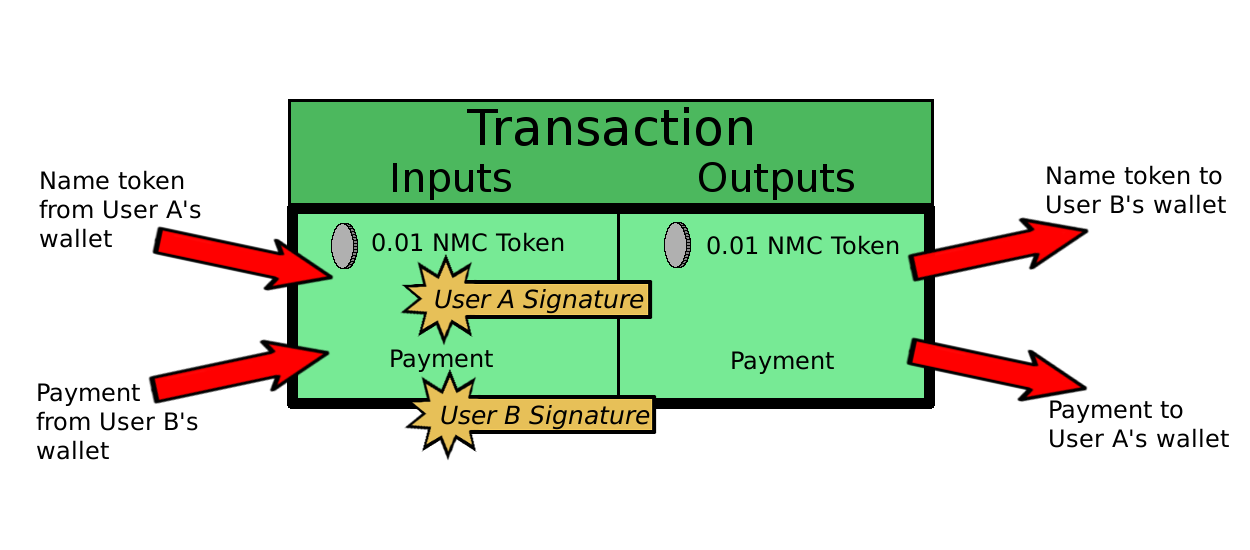
\includegraphics[width=0.9\textwidth]{figures/atomicTX}
  \caption{Anatomy of an atomic name transfer. Both the name and the payment are included in the same transaction, so one cannot fail to transfer to the other party without the other failing to transfer.}
  \label{fig:atomic}
\end{figure*}

The safest way to buy and sell Namecoin names is through the use of atomic transactions. This is an important technique in cryptocurrencies whereby two parties can exchange digital assets (such as a name in exchange for currency) without a trusted intermediary without either worrying that the other will abscond after receiving her half of the bargain. We show how these transactions work in Figure \ref{fig:atomic}. In an atomic transaction, Alice and Bob make their exchange in a single transaction. In the simplest form of atomic name transfer, Bob creates a transaction which transfers his payment to Alice and transfers `d/example' to him. He then sends this transaction to Alice, the owner of the name, who verifies it, signs, and broadcasts the transaction to the block chain. Both Alice and Bob's signatures are locked to the inputs and outputs of the transaction so neither input can be spent individually without the full transaction. This transaction provides cryptographic security to both Alice and Bob since either both the name and coins will be exchanged or nothing will. Although there is nothing inherently different looking about this transaction on the block chain, there are a few possible techniques to detect them by implementation quirks.

The Namecoin client is a fairly underdeveloped piece of software and thus there is no built-in method of performing atomic transactions. In order to accomplish this task, the Namecoin RPC client must be used from the command line. In order to simplify this task, a Namecoin developer created ANTPY \cite{antpy}, a piece of software to automate the creation of atomic transactions. This software has the quirk that the buyer's payment goes to the address that the seller held the name in. To find these transactions we queried the block chain for transactions with a {\tt NAME\_FIRSTUPDATE} or {\tt NAME\_UPDATE} input from the same address as a non name output. We then further reduced this set by eliminating transactions where the name stayed at the same address.

We searched throughout the history of the Namecoin block chain for transactions fitting this specification. Our query returned 13 transactions which we believe represent all transactions built by the ANTPY script. However this by no means represents all sales on the block chain. We next attempt to discover atomic transactions in a different way.

A implementation-agnostic method for detecting atomic name transfers is to find transactions that clearly use change addresses. This occurs when there are two non-name outputs in a transaction that has a name input. In this case the buyer did not want to pay all of his input to the seller and thus kept some for himself. This leaves the transaction with 3 outputs. Under normal circumstances, {\tt NAME\_UPDATE} transactions will only have two outputs, a name output and a change address. Thus every transaction with three outputs is very likely an atomic name transfer.

In the history of the Namecoin block chain, we found 6 transactions fitting this form. However 5 of the 6 were also detected by the previous (ANTPY) criterion.

The 14 atomic transactions which we detected are a lower bound for the number of name transfers. We are unable to query for all atomic transactions since if the buyer doesn't want any change from a purchase and the seller gives the buyer a new address to send payment to, the transaction is indistinguishable from a regular non-transferring name update.

\subsection{Deriving an upper bound on number of sales}

Following up on our lower bound from the previous section, we now derive an upper bound on the number of name sales using data from the block chain. Whereas atomic transactions, can (sometimes) be recognized simply from their contents, other name sale transactions are not recognizable. Here the payment could be a separate transaction or even made in a currency other than Namecoin. We would hope that we could detect changes in name ownership by looking at changes in which key owns a name. However, since the Namecoin client defaults to sending names to new addresses on update, there is no way to look at an update and tell whether or not a name is being transferred between owners.

In order to detect non-atomic transactions we must expand our view to the prior value of a name being updated. Certainly if the value does not change then the transaction is simply renewing the name, not transferring it. However considering all other transactions to be name transfers is far too conservative of a criterion. Users freely update the values of names whenever information in them becomes outdated.

\begin{figure}
  \centering
  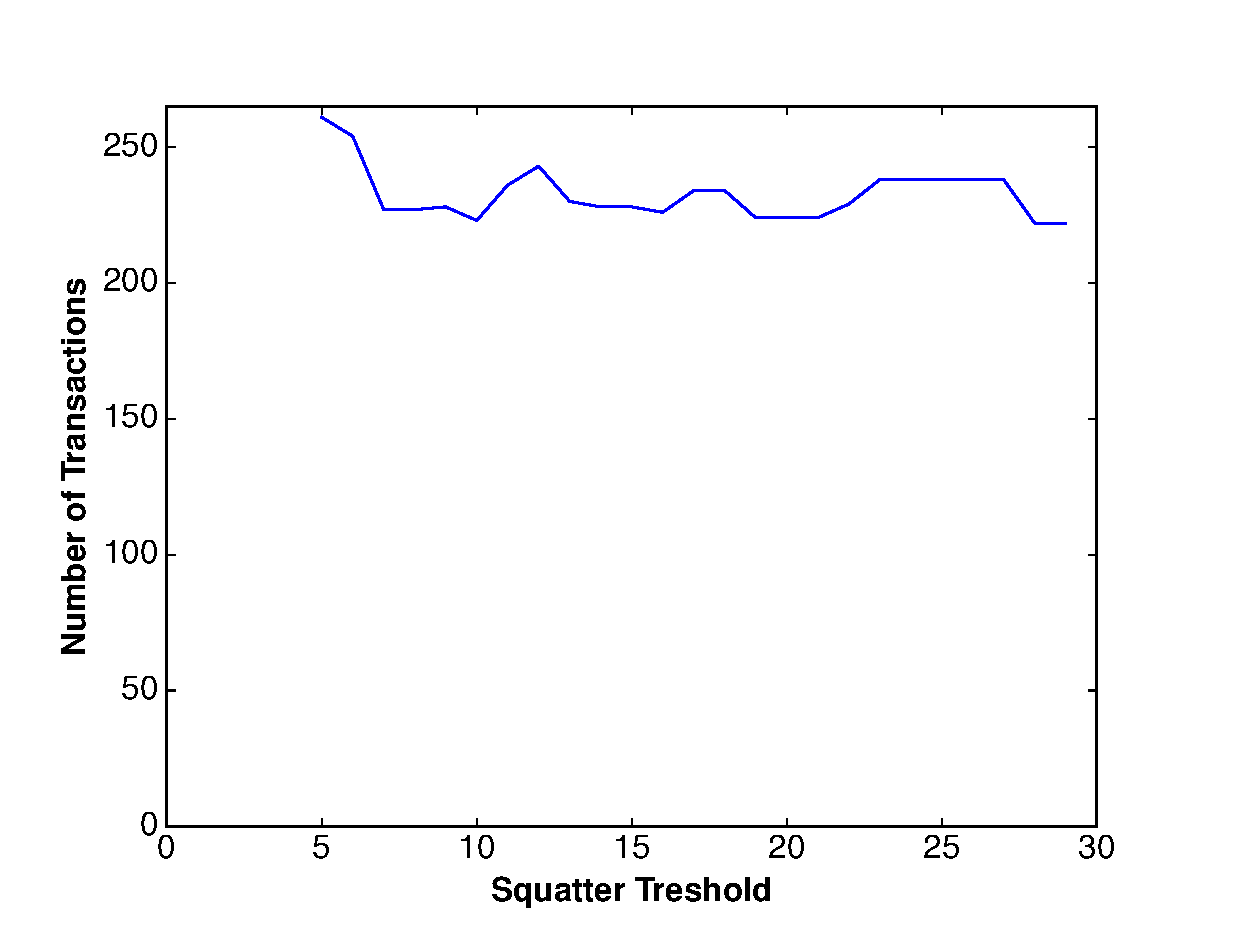
\includegraphics[width=0.9\columnwidth]{figures/transfers}
  \caption{Number of transfers detected based on squatting threshold. For each $n$ on the x-axis ($5 \leq n \leq 25$), we plot the number of squatter $\rightarrow$ non-squatter transactions detected if we characterize names whose values occur $n$ or more times as squatted.}
  \label{fig:percentSquatter}
\end{figure}

Although there doesn't seem to be a way to detect non-atomic name transfers generally, there is an important subclass of these transactions which can still be detected --- transfers from squatters to regular users. In the previous section we discussed our detection of squatters in the block chain which produces a list of values which with a high probability belong to squatters. Detecting transfers from squatters by finding names that change from one of these values to a value outside this set gives us a strategy to detect transfers.

We employ an additional criterion to eliminate false positives to tighten our upper bound. 
%Sometimes squatters update the value of their names, and thus a change from a squatter value may not represent the transfer of a name. To avoid picking up these updates as name transfers we restrict ourselves to selecting transactions that update the value of a name from a squatter value to a non-squatter value. 
If a name's value includes an info or email field and that stays the same in the updated value we can assume this is simply an update by the squatter. 

%Although this criterion is certainly not perfect, we believe that it has a fairly high success rate in revealing overall trends in name transfers.

Applying this analysis at various squatter threshold values, we see that the total number of squatter $\rightarrow$ non-squatter transactions detected holds at approximately 250 transactions. We emphasize that this value is likely an upper-bound since our criteria for reducing the number of transactions were quite conservative. 

To summarize, we would expect that given the high percentage of squatted .bit names, if there is a flourishing secondary market it would be dominated by sales from squatters to regular users. Yet we are able to upper bound the number of such transfers to about 250, a tiny fraction of the number of squatted names. Further, even though Namecoin supports a secure way to transfer names, we find strong evidence based on known tools supporting this functionality that its usage is very low.

\section{Analysis of Proposed Squatter Solutions}
\label{sec:analysis}

    Name squatting in Namecoin has been previously discussed as an issue facing the cryptocurrency. There have been several solutions proposed to alleviate the squatting issue by implementing new protocols or by placing additional fees on certain actions to either deter the actions of squatters or make it possible for a legitimate user to acquisition a desired name from a squatter if it increases the economic use of said name. In this section, we analyze some of the more popular methods, and discuss the costs to various individuals for each. 
    As it exists now, the only cost for an individual to register a name is the 0.01 NMC used to make the token, and then 0.01 NMC to cover two transactions fees (0.005 NMC each), one for the NAME\_NEW and one for the NAME\_FIRSTUPDATE transaction. Holding onto a name bares almost no cost with the owner only needing to pay 0.005 NMC as a transaction fee every time they post a NAME\_UPDATE transaction (which they need to do about once every 250 days). Losing a name doesn't cost a user anything, and the user gets gets the 0.01 NMC token back as a normal coin. 

\subsection{Adding a Cost to Updating Names}
    One of the most commonly suggested, and simplest, solutions to squatting is to add an associated fee with updating a name. The idea is that such a fee will not hinder a legitimate user very much, but will cause a squatter holding onto many domains to have to pay enough for the squatting to become financially infeasible. The reason that such a feature hasn't been implemented is because the Namecoin developers fear that the increased fees will disincentivise Namecoin adoption. Additionally, of the current squatters, some are benevolent and will give away names to users who have legitimate uses for the domains. Adding the renewal fees would punish these users who do not stand to gain monetarily from their efforts. This approach is very strong when it comes to deterring squatters who register thousands of domains. It is less effective against the type of squatter who registers just a few names that they think will be particularly valuable (like google.bit or poker.bit), or the type of squatter who is trying to squat on a name without the intent to sell, but just to hurt who they think the name would be valuable to.
For our analysis, we look into an update fee of 0.1 NMC. In this scenario, every time a user creates a NAME\_UPDATE transaction, a domain owner must burn 0.1 NMC for the transaction to be valid. Adding this fee wouldn't change the initial cost of registration, it would still be 0.02 NMC (0.01 from creating the token, and 2 transaction fees). The update fee will, however, change a user's cost on an update from 0.005 NMC to 0.105 NMC. Once the name expires, the user will again recoup their 0.01 NMC token that they attached to the name. 

\subsection{Varying Registration Costs Based on Name Lengths}
    Another commonly suggested solution is to vary the registration cost based on the length of the name. Shorter names are easier to remember, so the idea is they are generally worth more in practice and should cost more when they are registered. There have been various schemes suggested for the specifics on how the price should scale with name length, most of which resulting in exponentially decreasing costs for longer names. One issue with this approach is that the implicit assumption of this model, that shorter names are more valuable, may or may not actually reflect reality. Our results show that in the d/ namespace, more shorter names are taken, but this doesn't necessarily mean that they are more valuable. We speculate that a name like amazon.bit is probably more valuable than xyz.bit, and this wouldn't be reflected with this kind of pricing scheme.  This method does provide a good deterrent against squatters who are trying to claim many short names, but is rather ineffective against a squatter who is either trying to claim specific, valuable domain names, or hoard large quantities of longer domain names. 
    There exist many pricing protocols, but we have chosen to analyze the strategy outlined on the Namecoin Pricing wiki in more depth. According to this system, the prices depended on multipliers of an arbitrary price for different name lengths. 

\begin{figure*}
  \centering
  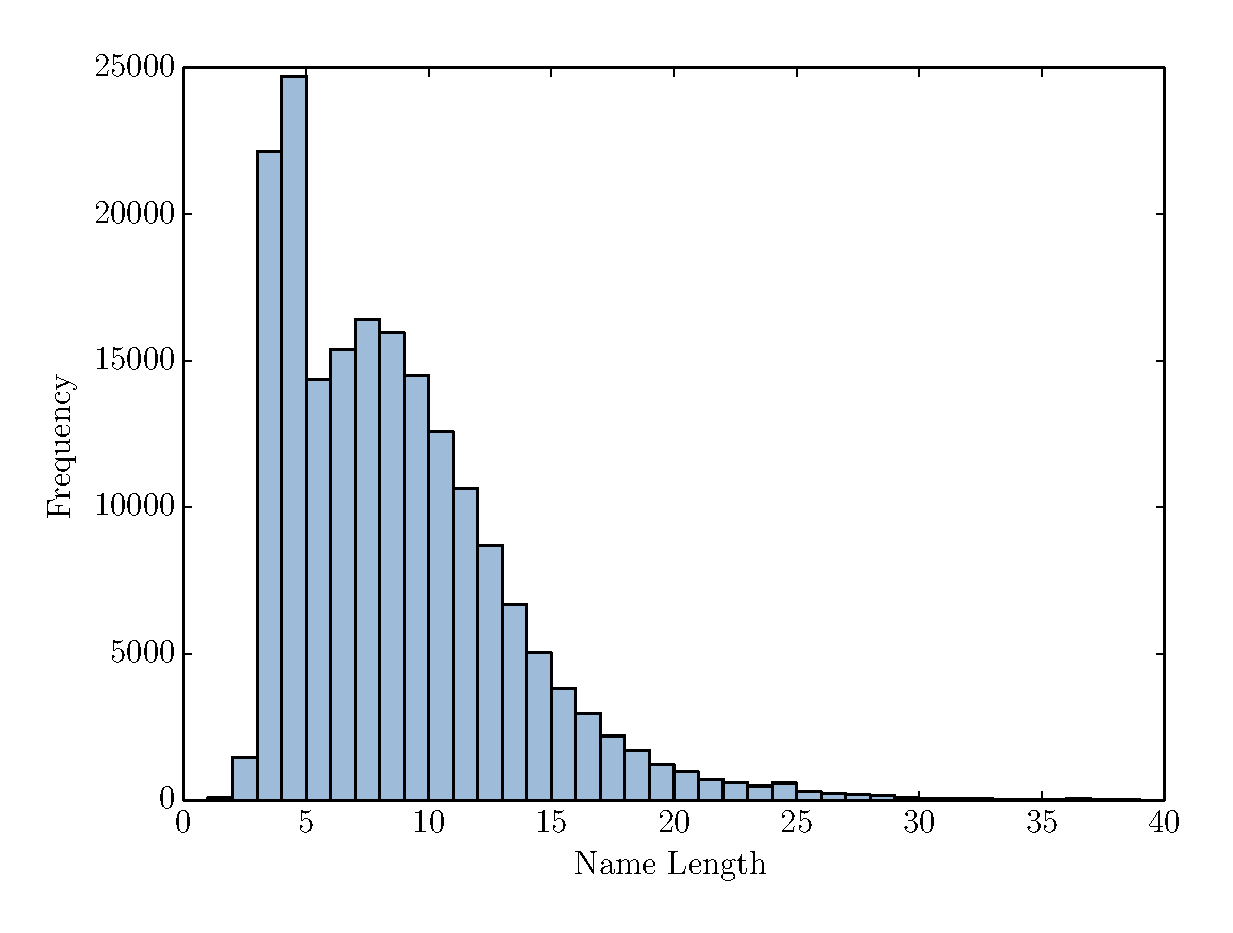
\includegraphics[width=0.95\textwidth]{figures/name_length_histogram}
  \caption{Length of Registered Names}
  \label{fig:nameLength}
\end{figure*}

\begin{table}[t]
  \centering
    \rowcolors{1}{}{lightgray}
  \begin{tabular}{| l | l |} \hline
    Length in Characters & Cost Multiplier \\
    1-3 & \( 5 x \) \\
    4-6 & \( 2 x \) \\
    7-14 & \( 1 x \) \\
    15-20 & \( \frac{1}{2} x \) \\
    21 + & minimum cost \\ \hline
  \end{tabular}
  \caption{Length based multipliers.}
\end{table}




    We use 0.5 NMC (could change) as the arbitrary price to be multiplied for our cost estimations. The update fees and the returned token are the same in this method as they are in the existing structure. The only change in cost is in the registration fee. In order to calculate what an average name would cost to register under this protocol, we have uniformly taken random names from the distribution of name length, and averaged the registration cost of these names. 



\subsection{Auctions}
    In this method for dealing with squatters, the Namecoin protocol could enforce that domain names are put up for auction on a periodic basis (perhaps every 52,000 blocks or about once/year). The protocol would allow for an auction after enough time has passed since the last auction, or since the NAME\_FIRSTUPDATE transaction for any given name. When an auction occurs, a name will become available and whomever is willing to pay the most for the domain name will get the name. In order to make it easier to retain a name, it has been suggested that the current owner should get some sort of advantage in the auction, so that the only need to bid some fraction of the highest bid in order to retain the name (let this be 1/100 for this discussion). If the current owner wins the auction, then they 'pay the network'. The cleanest way to do this is to burn the coins. Essentially, if the market cap of the currency doesn't change, then burning the coins from the auctions would uniformly increase the value of all the other remaining coins (burning too many coins can cause its own problems, too. Paying the network could also be done through other means, such as paying a random active address in the blockchain). The overall result should be that the fee paid for retaining a name should be spread out amongst other users of system. If, on the other hand, a new user wins the auction and bids more that 100 times the bid of the current owner of the name, the new user will gain the name, and the old owner will be the recipient of the auction coins. 
    An auction system like this has many disadvantages. The largest issue with this kind of squatting solution is that it erodes .bit's resistance to anti-censorship. One of the fundamental ideals of Namecoin and the .bit TLD is that it promotes freedom of speech, where a central authority is unable to censor content. Allowing a party to claim a domain as long as they are willing to pay enough undermines this concept. Periodic auctions would allow any large entity, such as an oppressive government, to easily seize names from any smaller entity that they want to silence. The counter argument here is that if a large entity seizes a smaller entities domain, the small entity would get paid a considerable sum-- in this case, 100 times what they were willing to bid to keep the domain. Whether or not the cash received by the censoring of the domain is worth more to the small entity than having the domain is a question that we do not explore.  An additional weakness of this system is that it can cause a legitimate user to have to pay lots of money in order to keep their domain every auction. Even with a large advantage, if owning a particular .bit domain is of great importance to an individual, then they can be forced to pay a large sum of money every auction. If "Business" is trying to hold onto business.bit, and business.bit is worth a considerable amount to them (say they get many online sales there), then a competitor to Business could bid some factor  less than what business.bit is worth to Business. Business isn't willing to part with business.bit for this amount of money, so they are forced to instead pay 1\% of what business.bit is worth every time there is an auction for their domain.
    Under this model, the initial cost a domain depends on how an individual acquires the domain. If they acquire the domain without an auction, then the cost is the same as it is in the existing protocol. Conversely, if an entity acquires a domain through the auction process, then the fee they will need to pay will depend on the value of the domain to whomever they are buying it from. If the seller is a squatter, the buyer will need to bid an amount equal to what the squatter thinks the domain is worth (the squatter will bid 1\% of what they think the domain is worth). Holding onto a domain in this model can be expensive; as discussed previously, every time there is an auction, the owner of a domain can be forced into paying 1\% of what the domain is worth to them, which could be a sizeable amount of money. Aside from the auction costs, there is still the small transaction fee that the owner will need to pay for every NAME\_UPDATE transaction. If a user lets their name expire, this situation is identical to the ones previously discussed, but if an individual loses control of a name because of an auction, they don't get their 0.01 NMC token back and they instead get the money from the auction. In this case, they receive an amount of money equal to the value of the domain to them. 

\subsection{Require an Escrow}
    Another proposed solution is to require a number of namecoins to be put into an escrow account when claiming a name. The money in escrow would be locked, so that the owner of the name is unable to spend that money, but once the owner loses or forfeits the name, the money in escrow is returned. The exact amount of money to be put into escrow is a debated topic. In one such model, the amount is decided by the owner of the name. In this situation, there would be an additional protocol designed to allow someone to take a name if they are willing to pay more money into an escrow account for said name than the current owner. If someone tries to place more money into escrow than the current owner (in an attempt to take the name), the current owner is notified and has a short grace period in which they can protect themselves by placing a larger amount of money in the escrow account. In order to prevent the the same problems and censorship erosion as seen in the case with auctions, there is a maximum allowed escrow and once a domain owner fills the escrow to this amount, the name becomes locked and it would be impossible for another user to seize for any amount of money (let this maximum value be 200 NMC). This provides reasonable financial protection against squatters who are trying to squat on thousands of domains, because a squatter such as this would need to fill the escrows for any of the domains that they are squatting that other people want. If a user out-escrows a squatter, this represents an ultimate failure in the eyes of the squatter because they lose the domain name and get paid nothing. The only way for a squatter to prevent this is to continue to fill their escrows for names that a user wants until the escrows are full. Once the squatter puts money into escrow, they can't remove it without losing the name, so eventually all of the escrows for all of the names users want would need to be full. This penalizes certain squatters more than others, in the sense that the squatter will always eventually get their coins back. A squatter that doesn't need access to their coins has no issue with locking up some huge fraction of them in escrow, because they will eventually get the coins back. A poorer squatter, on the other hand, who doesn't have enough coins to have some of them locked up for every domain they try to squat, will be forced to stop. 
    The cost of registering a name is now variable because a user can decide how much or little money they want to put into escrow. This has the advantage of being acceptable to many different types of users. A serious user who is only interested in having a few valued domains and doesn't want to risk losing their domains can easily pay to fill an escrow account for their domains. At the same time, a more casual user, who just wants some domain (but not a valuable domain) can still attain this domain while only owning a small number of coins. The cost of holding onto a domain is the same as it is in the present situation. Once a domain name is lost, a user will gain access to all the money locked into escrow for that name.     

\subsection{Cost Analysis}
    In order to compare the overall costs of the various models, we consider applying the cost assumptions outlined above to different users trying to hold onto domains for a period of 3 years. One user is a squatter who is trying to hold on to 1000 domains of variable length and value. Another is a squatter who is only trying to squat 5 particularly valuable names. The final two a legitimate users, one of which is looking to use a very specific, valued domain name, and the other is a user that just wants a domain, but doesn't really care what the domain is.


\begin{table*}[t]
  \centering
  \rowcolors{3}{}{lightgray}
  \begin{tabularx}{\linewidth}{| X | X | X | X | X |} \hline
    &  Squatter with 1000 domains & Squatter with a few valuable domains & User who wants any domain & User who wants a specific, valuable domain\\
\hline
    \multicolumn{5}{|c|}{\textbf{Registration Cost}} \\ \hline
Current System &  20 NMC & 0.1 NMC & 0.02 NMC & 0.02 NMC, or best offer from squatter \\
Increasing Update fee & 20 NMC & 0.1 NMC & 0.1 NMC & 0.02 NMC \\
Length based fees & 737.77 & 3.68 & 0.74 & 0.74 \\ 
Auctions & 20 NMC & 0.1 NMC & 0.1 NMC & Fee paid in Auction \\
Escrow & 200,000 NMC & 1,000 NMC & 0.02 NMC & 200 NMC \\ \hline

\multicolumn{5}{|c|}{\textbf{Longer term cost (3 years of Updates)}} \\ \hline
Current & 25 NMC & 0.125 NMC & 0.025 NMC & 0.025 NMC \\ 
Increasing Update fee & 500 NMC & 2.5 NMC & 0.5 NMC & 0.5 NMC \\ 
Length based fees & 25 NMC & 0.125 NMC & 0.025 NMC & 0.025 NMC \\ 
Auctions & & & 1 \% of what domain is worth to user & 1 \% of what domain is worth to user \\ 
Escrow & 25 NMC & 0.125 NMC & 0.025 NMC & 0.025 NMC \\ \hline

\multicolumn{5}{|c|}{\textbf{Refund Upon Losing Name}} \\ \hline
Current & 10 NMC & 0.05 NMC & 0.01 NMC & 0.01 NMC \\
Increasing Update fee & 10 NMC & n0.05 NMC & 0.01 NMC & 0.01 NMC \\
Length based fees & 10 NMC & 0.05 NMC & 0.01 NMC & 0.01 NMC \\
Auctions & & & What the domain is worth to user & What the domain is worth to user \\ \hline
  \end{tabularx}
  \caption{Cost comparison of the various anti-squatter mechanisms.}
\end{table*}



\section{Results}
\label{sec:results}

So far in this paper we have described the market behavior in the Namecoin system. Now we create a predictive model for analyzing the value of names. We explore a number of factors useful in predicting name values. For each factor we describe what affect it has on name value, and how this is similar or different from the standard domain system.

\textbf{Alexa Ranking:} The popularity of a domain under the standard ICANN system should be suggestive of a dot bit domain's popularity
\section{Related Work}
\label{sec:related}

Here we discuss attempts besides Namecoin at decentralized cryptocurrency-based namespaces or domain-name systems and more broadly in technologies that utilize the block chain.

Bitshares is another altcoin that includes proposals for a namespace as one of its goals \cite{bitsharesdns}. Emercoin recently emerged as a Namecoin competitor \cite{emercoin}. 

More broadly, the ability to publish messages to the block chain immediately allows a variety of applications. Physical property, shares of stocks, bonds, or any other real asset can be digitally represented on the block chain. Overlay protocols such as Mastercoin and Colored Coins specify a syntax and semantics for such digital representations \cite{mastercoinspec, rosenfeld2012overview}. CommitCoin allows for putting hash commitments on the Bitcoin block chain in order to timestamp data in a trustless manner \cite{clark2012commitcoin}.

There are a number of more complex applications that require additional primitives. Financial derivatives are contracts whose value depends, in some mutually agreed-upon way, on the price (or movements in price) of an underlying asset. Implementing derivatives of digital assets, then, requires user-defined logic (or scripts) for transaction validation. This can be accomplished via an altcoin with a flexible scripting language such as Ethereum \cite{ethereumwhitepaper}. Furthermore, since derivatives depend on prices, scripts that implement them require access to price feeds as input. Otherwise, it requires a trusted third party (known by a Bitcoin address) to regularly publish suitably encoded, signed price statements reflecting external reality. These can be published directly to the block chain or distributed off-chain and only added to the block chain when needed to redeem an asset. More generally, such entities could publish any data feed representing news or other events.

Bitcoin can act as a platform for fair secure multiparty computation \cite{andrychowicz2014secure, bentov2014use, kumaresan2014use}. These are SMC protocols augmented with Bitcoin operations, e.g., a payment from one participant to another, or a deposit.

Finally, a set of related ideas known as decentralized autonomous organizations (among several other names) has stirred considerable excitement in the community recently. These combine several primitives discussed above --- digital assets, long-lived scripts implementing arbitrary logic governing those assets, data feeds, and out-of-band communication. Some proposals for DAOs incorporate human input in various forms: one is a decentralized agent farming out computationally intractable tasks to humans \cite{buterindao}. Another is voting by shareholders of decentralized agents to enable modifications to the logic (i.e., script). 

% As with any input external to the block chain, these must be implemented using data feeds.

% The block chain has been proposed as a stratum for building technologies and mechanisims beyond storing financial transactions. Hash commitments appear in the Namecoin protocol for registering new names. In  \cite{bonneau2014decentralizing} the authors describe how to use the block chain to create prediction markets and order books.

\section{Conclusion}
\label{sec:conclusion}


%% Bibliography
%\vspace{-1ex}
%\linespread{1.0}
%\setlength{\bibsep}{1pt}
%\footnotesize
\small
\bibliographystyle{unsrtnat}
% \bibliographystyle{abbrvnat}
\bibliography{local}


\end{document}

